\documentclass[12pt,]{article}
\usepackage{lmodern}
\usepackage{amssymb,amsmath}
\usepackage{ifxetex,ifluatex}
\usepackage{fixltx2e} % provides \textsubscript
\ifnum 0\ifxetex 1\fi\ifluatex 1\fi=0 % if pdftex
  \usepackage[T1]{fontenc}
  \usepackage[utf8]{inputenc}
\else % if luatex or xelatex
  \ifxetex
    \usepackage{mathspec}
  \else
    \usepackage{fontspec}
  \fi
  \defaultfontfeatures{Ligatures=TeX,Scale=MatchLowercase}
    \setmainfont[]{Times}
\fi
% use upquote if available, for straight quotes in verbatim environments
\IfFileExists{upquote.sty}{\usepackage{upquote}}{}
% use microtype if available
\IfFileExists{microtype.sty}{%
\usepackage{microtype}
\UseMicrotypeSet[protrusion]{basicmath} % disable protrusion for tt fonts
}{}
\usepackage[margin=1in]{geometry}
\usepackage{hyperref}
\hypersetup{unicode=true,
            pdftitle={I.C.Y Report},
            pdfborder={0 0 0},
            breaklinks=true}
\urlstyle{same}  % don't use monospace font for urls
\usepackage{graphicx,grffile}
\makeatletter
\def\maxwidth{\ifdim\Gin@nat@width>\linewidth\linewidth\else\Gin@nat@width\fi}
\def\maxheight{\ifdim\Gin@nat@height>\textheight\textheight\else\Gin@nat@height\fi}
\makeatother
% Scale images if necessary, so that they will not overflow the page
% margins by default, and it is still possible to overwrite the defaults
% using explicit options in \includegraphics[width, height, ...]{}
\setkeys{Gin}{width=\maxwidth,height=\maxheight,keepaspectratio}
\IfFileExists{parskip.sty}{%
\usepackage{parskip}
}{% else
\setlength{\parindent}{0pt}
\setlength{\parskip}{6pt plus 2pt minus 1pt}
}
\setlength{\emergencystretch}{3em}  % prevent overfull lines
\providecommand{\tightlist}{%
  \setlength{\itemsep}{0pt}\setlength{\parskip}{0pt}}
\setcounter{secnumdepth}{0}
% Redefines (sub)paragraphs to behave more like sections
\ifx\paragraph\undefined\else
\let\oldparagraph\paragraph
\renewcommand{\paragraph}[1]{\oldparagraph{#1}\mbox{}}
\fi
\ifx\subparagraph\undefined\else
\let\oldsubparagraph\subparagraph
\renewcommand{\subparagraph}[1]{\oldsubparagraph{#1}\mbox{}}
\fi

%%% Use protect on footnotes to avoid problems with footnotes in titles
\let\rmarkdownfootnote\footnote%
\def\footnote{\protect\rmarkdownfootnote}

%%% Change title format to be more compact
\usepackage{titling}

% Create subtitle command for use in maketitle
\providecommand{\subtitle}[1]{
  \posttitle{
    \begin{center}\large#1\end{center}
    }
}

\setlength{\droptitle}{-2em}

  \title{I.C.Y Report}
    \pretitle{\vspace{\droptitle}\centering\huge}
  \posttitle{\par}
    \author{}
    \preauthor{}\postauthor{}
      \predate{\centering\large\emph}
  \postdate{\par}
    \date{19 August, 2019}

\usepackage{graphicx}

\usepackage {hyperref}
\hypersetup {colorlinks = true, linkcolor = cyan, urlcolor = cyan}
\usepackage[font={small}, labelfont={bf}]{caption}
\usepackage{fancyhdr}
\usepackage{float}
\usepackage{longtable, tabu}
\usepackage{booktabs}
\usepackage{makecell}
\usepackage[table]{xcolor}
\usepackage{pdflscape}
\usepackage[export]{adjustbox}

\begin{document}
\maketitle

~ ~ ~ ~

\vspace{4cm}

\begin{figure}[H]


\includegraphics[width=\linewidth]{../Images/logo.png}
 
\end{figure}

\clearpage

\section{\textbf{How to use this report}}

The following report uses studbook data to generate tables and plots
designed to help practitioners choose which individuals would be most
suitable to translocate to Mauritius. The suitability of a individual
for translocation is based on (1) the number of
\hyperlink{term0}{founder equivalents (Fe)} in an individual, and its
(2) \hyperlink{term2}{mean kinship coefficient (MK)}, which is a measure
of a individuals average relatedness to other individuals in the
population.

Founder equivalents are a way of measuring genetic diversity from
pedigree data. They can be thought as how many wild caught founders
would be needed to recreate the current level of genetic diversity and
can be calculated for individuals or for the population as a whole.
Founder equivalents is a metric that takes into account both the number
of founder genomes that an individual is descended from and also each
founder's relative contributions (or
\hyperlink{term1}{\textbf{founder representation}}). It is perhaps
intuitive that the more founders an individual is descended from the
greater its genetic diversity. However the relative contribution of each
of the founders is incredibly important as uneven contributions lead to
a loss in genetic diversity and an increase in inbreeding. The maximum
number of founder equivalents that an individual could have would be
equal to the number of individuals that founded the population
(according to the studbook) and would only occur if all of the founders
were represented evenly within that individual.

\textbf{Figure 1} gives a simple example of how founder representation
is calculated, it also demonstrates how this can be graphically
represented, \textbf{figure 2} gives an example demonstrating how graphs
of even and uneven founder representations may look.

\begin{figure}[H]

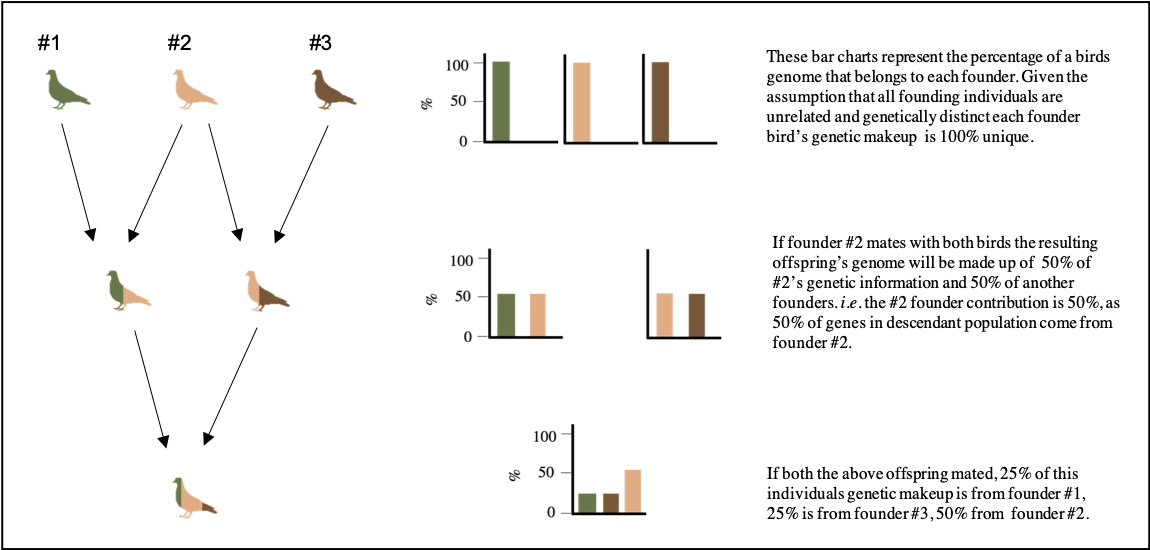
\includegraphics[width=\linewidth]{../Images/figure1.png}
  \caption{An example of how founder representation is calculated and how it can be visualised with bar charts}
\end{figure}

\begin{figure}[H]

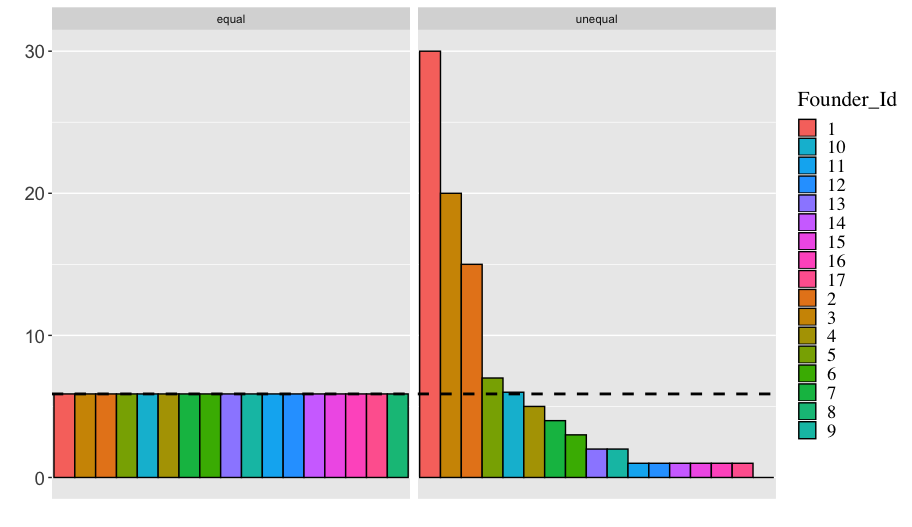
\includegraphics[width=0.7\linewidth, center]{../Images/figure2.png}
  \caption{An example of how equal and unequal founder representation graphs may look. The dashed line represents the expected height of the bars if founder representation was equal which in this example, with 17 founders, is 5.88\%}
\end{figure}

\subsection{\underline{\textbf{How to choose individuals for reintroduction}}}

This report should make it easier to choose individuals based on their
possible genetic diversity and relatedness however the rankings do not
include any other information that may, or may not, make an individual
suitable for reintroduction. Ultimately it will be up to the person
reading this report to decide what other factors (other than genetic
ones) make a individual suitable for translocation. The points below
provide further guidance for selecting individuals to maximise genetic
diversity in the released individuals and ensuring the overall genetic
health of the captive and released populations.

\begin{itemize}
\item \textbf{Highest ranking individuals.}\newline 
\item \textbf{Pragmatic considerations} - Age, locatation, possible disease or health issues, are the individuals available for translocations?\newline  
\item \textbf{How valuable are the individuals to the captive population?}- When you remove a individual from captivity you remove its genes and so a balance must be struck between translocating individuals and ensuring a heatlhy captive population that can continue to produce heatlhy, genetically diverse individuals for future reintroductions. Therefore it may be better to initially choose slightly lower ranking individuals because they will still have a positive impact on the wild population but will ensure a healthy, useful captive population.\newline
\item \textbf{How inbred are the individuals?} - The more inbred a individual the lower its genetic diversity and the greater the likelihood it will suffer from inbreeding depression. Inbreeding is measured by the \hyperlink{term4}{inbreeding coefficient}.\newline
\item \textbf{How related are the individuals to any that may have been previously translocated into the wild?}- This may not be relevant for the very first translocation but should be considered in any future translocations.\newline
\item \textbf{Make sure to select an even number of males and females.} - An uneven sex ratio during reintroductions has been shown to contribute to decreased genetic diversity and increased inbreeding.\newline 
\end{itemize}

\section{\underline{\textbf{Report Contents}}}

All section titles below (in blue) are linked directly to the sections
they refer to (just click on them!), any words in blue link to the
glossary at the end of the report, any references in blue are
hyperlinked to the relevant manuscripts URLs.

\subsection{\underline{\textbf{Main reports}}}

\hyperlink{found_contrib}{\textbf{Founder representation report}} -
Summary of the numer of founder equivalents in the current population
and a bar chart which shows what proportion of the genes in the current
population come from each founder (founder representation). This gives
an indication of the overall genetic health of the captive population
and which founders may be under-represented and therefore whose genetic
contribution is in danger of being lost from the population.

\hyperlink{best_ind}{\textbf{Individuals recommended for reintroduction}}
- Table with group of individuals most suitable for reintroduction based
on ICYs algorithm (group of birds least related with most Fe, lowest
MK). Graphs showing founder contribution of the chosen animals and how
it compares with the overall founder represention with the population as
a whole.

\subsection{\underline{\textbf{Supplementary reports}}}

\hyperlink{fem_rep}{\textbf{Female suitability report}} - Bar charts of
founder representation for each living female individual in the
population, this is followed by a spreadsheet showing the ranks of
females based on the number of founder equivalents and mean kinship
coefficient.

\hyperlink{male_rep}{\textbf{Male suitability report}} -Bar charts of
founder representation for each living male individual in the
population, this is followed by a spreadsheet showing the ranks of males
based on the number of founder equivalents and mean kinship coefficient.

\hyperlink{overall}{\textbf{Overall suitability report}}- Spreadsheet of
most to least suitable individuals to supplement (regardless of sex),
including more details about founder representations.

\subsection{\underline{\textbf{Glossary \& references}}}

\hyperlink{terms}{\textbf{Glossary}}- Provides definitions of a few key
terms (found in blue throughout the report)

\hyperlink{reading}{\textbf{Recommended reading \& references}} -
Suggestions for further reading and references that contributed to this
report.

\begin{center}\rule{0.5\linewidth}{\linethickness}\end{center}

\clearpage
\hypertarget{found_contrib}{\section{\textbf{Founder representation report}}}

\subsection{\underline{\textbf{Summary}}}

The number of founders represented in the population is 17, if the
founders were all represented evenly they would be present at 5.88\%
within the population.The number of founder equivalents found on average
in the population could be increased by tactical breeding to even out
representations.\newline
\subsection{\underline{\textbf{Founder representation in the current population}}}
The graph below shows how each founder is represented in the current
population the dashed line represents the expected height of the bars if
founder representation is equal 5.88. For example it can be seen that
the highest proportion of genes in the current population belong to
individual 13 . In contrast only a small proportion of the genes present
in todays population come from founder 132. This may mean that the
population could be in danger of losing all genes from 132 unless
careful attention is paid in the following breeding seasons to maximise
132 contribution to the population. If a founders' contribution is lost
from the population, that population loses genetic diversity and will
likely be less healthy and robust.\newline 

\includegraphics{ICY_files/figure-latex/unnamed-chunk-4-1.pdf}

\newpage

\hypertarget{best_ind}{\section{\textbf{Individuals recommended for reintroduction}}}

The table below contains the individuals that are recommended for
reintroduction. These individuals are not just the highest ranked but
are the highest ranked individuals that as a group of individuals are
the least related. The rankings are based on the individuals mean
kinship and the number of founders in their genome however it is
important that the group of individuals being released are as unrelated
as possible to avoid inbreeding depression and increase genetic
diversity. The graphs show the founder representation of each bird (bar
chart) and the line shows how the different founders are represented in
the population as a whole (this the same data as represnted in the
founder representation bar chart on the previous page).

\begin{longtable}{rlllrrrrr}
\caption{\label{tab:unnamed-chunk-5}individuals recommended for reintroduction/translocation.}\\
\toprule
\textbf{Rank} & \textbf{UniqueID} & \textbf{Location} & \textbf{Sex} & \textbf{F} & \textbf{MK} & \textbf{AgeYears} & \textbf{Number of founders} & \textbf{Fe}\\
\midrule
\endfirsthead
\caption[]{individuals recommended for reintroduction/translocation. \textit{(continued)}}\\
\toprule
\textbf{Rank} & \textbf{UniqueID} & \textbf{Location} & \textbf{Sex} & \textbf{F} & \textbf{MK} & \textbf{AgeYears} & \textbf{Number of founders} & \textbf{Fe}\\
\midrule
\endhead
\
\endfoot
\bottomrule
\endlastfoot
\rowcolor{gray!6}  2 & 1456 & JERSEY & Male & 0.039 & 0.124 & 10 & 16 & 14.254\\*
\end{longtable}

\includegraphics{ICY_files/figure-latex/unnamed-chunk-5-1.pdf}

\newpage

\hypertarget{fem_rep}{\section{\textbf{Female suitability report}}}

The bar charts below shows the founder representation for each female
indiviudal in the current population. The Unique ID for a individual is
at the top of each plot and the dashed line represents the expected
height of the bars if founder representation is equal (5.88\%). The
graphs are arranged from highest ranking individual (top left) to lowest
ranking individual (bottom right). The page after the graphs contains a
table detailing the highest to lowest ranked female individuals (all
rankings based on the number of founder equivalents (Fe) and mean
kinship coefficients (MK)).The table also contains information that may
be useful when selecting individuals for translocation such as age,
location of zoo \& \hyperlink{term4}{inbreeding coefficient} (F)
.\newline  

~ ~ ~

\includegraphics{ICY_files/figure-latex/unnamed-chunk-6-1} \newpage

\begin{longtable}{ccccccc>{\centering\arraybackslash}p{5em}c}
\caption{\label{tab:unnamed-chunk-7}Information of females most to least suitable for translocation, rankings based on the number of founder equivalents (Fe) in an individual and its mean kinship (MK)}\\
\toprule
\textbf{Rank} & \textbf{UniqueID} & \textbf{Location} & \textbf{Sex} & \textbf{F} & \textbf{MK} & \textbf{AgeYears} & \textbf{Number of founders} & \textbf{Fe}\\
\midrule
\endfirsthead
\caption[]{Information of females most to least suitable for translocation, rankings based on the number of founder equivalents (Fe) in an individual and its mean kinship (MK) \textit{(continued)}}\\
\toprule
\textbf{Rank} & \textbf{UniqueID} & \textbf{Location} & \textbf{Sex} & \textbf{F} & \textbf{MK} & \textbf{AgeYears} & \textbf{Number of founders} & \textbf{Fe}\\
\midrule
\endhead
\
\endfoot
\bottomrule
\endlastfoot
\rowcolor{gray!6}  1 & 1388 & SD-WAP & Female & 0.039 & 0.111 & 13 & 16 & 14.254\\
3 & 1704 & PRAHA & Female & 0.068 & 0.144 & 1 & 17 & 14.030\\
\rowcolor{gray!6}  6 & 1801 & JERSEY & Female & 0.068 & 0.144 & 0 & 17 & 14.030\\
10 & 1554 & KOLN & Female & 0.074 & 0.115 & 6 & 17 & 14.011\\
\rowcolor{gray!6}  14 & 1610 & FARNHAM & Female & 0.074 & 0.136 & 2 & 17 & 14.011\\
\addlinespace
18 & 1612 & CHESTER & Female & 0.075 & 0.156 & 2 & 17 & 13.357\\
\rowcolor{gray!6}  20 & 1614 & FARNHAM & Female & 0.075 & 0.156 & 2 & 17 & 13.357\\
21 & 1618 & KOLN & Female & 0.075 & 0.156 & 2 & 17 & 13.357\\
\rowcolor{gray!6}  22 & 1619 & MULHOUSE & Female & 0.075 & 0.156 & 2 & 17 & 13.357\\
25 & 1703 & PRAHA & Female & 0.075 & 0.156 & 1 & 17 & 13.357\\
\addlinespace
\rowcolor{gray!6}  26 & 1728 & JERSEY & Female & 0.075 & 0.156 & 1 & 17 & 13.357\\
27 & 1729 & JERSEY & Female & 0.075 & 0.156 & 1 & 17 & 13.357\\
\rowcolor{gray!6}  28 & 1739 & JERSEY & Female & 0.075 & 0.156 & 1 & 17 & 13.357\\
30 & 1807 & JERSEY & Female & 0.075 & 0.156 & 0 & 17 & 13.357\\
\rowcolor{gray!6}  32 & 1815 & JERSEY & Female & 0.075 & 0.156 & 0 & 17 & 13.357\\
\addlinespace
40 & 1827 & FARNHAM & Female & 0.184 & 0.140 & 0 & 17 & 13.169\\
\rowcolor{gray!6}  41 & 1833 & FARNHAM & Female & 0.184 & 0.140 & 0 & 17 & 13.169\\
43 & 1707 & FARNHAM & Female & 0.184 & 0.141 & 1 & 17 & 13.169\\
\rowcolor{gray!6}  44 & 1839 & JERSEY & Female & 0.181 & 0.162 & 0 & 17 & 13.048\\
45 & 1847 & JERSEY & Female & 0.181 & 0.162 & 0 & 17 & 13.048\\
\addlinespace
\rowcolor{gray!6}  48 & 1803 & WILDPLACE & Female & 0.072 & 0.128 & 0 & 17 & 12.837\\
51 & 1853 & FARNHAM & Female & 0.071 & 0.138 & 0 & 17 & 12.388\\
\rowcolor{gray!6}  55 & 1731 & JERSEY & Female & 0.204 & 0.169 & 1 & 17 & 12.016\\
56 & 1736 & JERSEY & Female & 0.204 & 0.172 & 1 & 17 & 12.016\\
\rowcolor{gray!6}  58 & 1738 & JERSEY & Female & 0.204 & 0.174 & 1 & 17 & 12.016\\
\addlinespace
60 & 1814 & JERSEY & Female & 0.372 & 0.176 & 0 & 17 & 12.016\\
\rowcolor{gray!6}  65 & 1604 & JERSEY & Female & 0.093 & 0.158 & 3 & 17 & 11.945\\
67 & 1481 & BURFORD & Female & 0.045 & 0.136 & 10 & 15 & 11.939\\
\rowcolor{gray!6}  70 & 1589 & JERSEY & Female & 0.065 & 0.170 & 4 & 17 & 11.921\\
71 & 1596 & JERSEY & Female & 0.065 & 0.174 & 4 & 17 & 11.921\\
\addlinespace
\rowcolor{gray!6}  72 & 1706 & MULHOUSE & Female & 0.080 & 0.112 & 1 & 17 & 11.872\\
74 & 1575 & JERSEY & Female & 0.349 & 0.117 & 5 & 15 & 11.058\\
\rowcolor{gray!6}  77 & 1622 & NY BRONX & Female & 0.063 & 0.104 & 2 & 13 & 10.512\\
79 & 1441 & JERSEY & Female & 0.158 & 0.115 & 11 & 15 & 10.304\\
\rowcolor{gray!6}  82 & 1720 & WILDPLACE & Female & 0.082 & 0.129 & 1 & 17 & 10.127\\
\addlinespace
83 & 1721 & PAIGNTON & Female & 0.082 & 0.129 & 1 & 17 & 10.127\\
\rowcolor{gray!6}  84 & 1805 & WILDPLACE & Female & 0.082 & 0.129 & 0 & 17 & 10.127\\
87 & 1719 & CHESTER & Female & 0.082 & 0.130 & 1 & 17 & 10.127\\
\rowcolor{gray!6}  88 & 1620 & WILDPLACE & Female & 0.082 & 0.131 & 2 & 17 & 10.127\\
89 & 1630 & BURFORD & Female & 0.082 & 0.131 & 2 & 17 & 10.127\\
\addlinespace
\rowcolor{gray!6}  90 & 1536 & NY BRONX & Female & 0.123 & 0.110 & 7 & 16 & 9.909\\
91 & 1588 & NY BRONX & Female & 0.123 & 0.110 & 5 & 16 & 9.909\\
\rowcolor{gray!6}  92 & 1615 & SD-WAP & Female & 0.123 & 0.110 & 2 & 16 & 9.909\\
93 & 1624 & SD-WAP & Female & 0.123 & 0.110 & 2 & 16 & 9.909\\
\rowcolor{gray!6}  94 & 1734 & SD-WAP & Female & 0.123 & 0.110 & 1 & 16 & 9.909\\
\addlinespace
95 & 1746 & SD-WAP & Female & 0.123 & 0.110 & 1 & 16 & 9.909\\
\rowcolor{gray!6}  98 & 1810 & CHESTER & Female & 0.107 & 0.116 & 0 & 17 & 9.295\\
99 & 1392 & NY BRONX & Female & 0.065 & 0.095 & 13 & 13 & 9.220\\
\rowcolor{gray!6}  101 & 1496 & NY BRONX & Female & 0.094 & 0.097 & 9 & 14 & 8.380\\
102 & 1464 & WILDPLACE & Female & 0.144 & 0.118 & 10 & 8 & 7.940\\
\addlinespace
\rowcolor{gray!6}  103 & 1351 & NY BRONX & Female & 0.102 & 0.112 & 14 & 8 & 7.912\\
105 & 1379 & NY BRONX & Female & 0.092 & 0.091 & 14 & 8 & 7.077\\
\rowcolor{gray!6}  107 & 1416 & NY BRONX & Female & 0.078 & 0.097 & 11 & 9 & 6.832\\
110 & 1203 & TRACY AV & Female & 0.179 & 0.102 & 20 & 8 & 5.884\\*
\end{longtable}\newpage

\hypertarget{male_rep}{\section{\textbf{Male suitability report}}}

The bar charts below shows the founder representation for each male
indiviudal in the current population. The Unique ID for a individual is
at the top of each plot and the dashed line represents the expected
height of the bars if founder representation is equal (5.88\%). The
graphs are arranged from highest ranking individual (top left) to lowest
ranking individual (bottom right). The page after the graphs contains a
table detailing the highest to lowest ranked male individuals (all
rankings based on the number of founder equivalents (Fe) in an
individual and its mean kinship coefficients (MK)).The table also
contains information that may be useful when selecting individuals for
translocation such as age, location of zoo \&
\hyperlink{term4}{inbreeding coefficient} (F) value.\newline   ~ ~ ~

\includegraphics{ICY_files/figure-latex/unnamed-chunk-8-1}

\newpage

\begin{longtable}{ccccccc>{\centering\arraybackslash}p{5em}c}
\caption{\label{tab:unnamed-chunk-9}Information of females most to least suitable for translocation, rankings based on the individual founder equivalent (Fe) and mean kinship (MK)}\\
\toprule
\textbf{Rank} & \textbf{UniqueID} & \textbf{Location} & \textbf{Sex} & \textbf{F} & \textbf{MK} & \textbf{AgeYears} & \textbf{Number of founders} & \textbf{Fe}\\
\midrule
\endfirsthead
\caption[]{Information of females most to least suitable for translocation, rankings based on the individual founder equivalent (Fe) and mean kinship (MK) \textit{(continued)}}\\
\toprule
\textbf{Rank} & \textbf{UniqueID} & \textbf{Location} & \textbf{Sex} & \textbf{F} & \textbf{MK} & \textbf{AgeYears} & \textbf{Number of founders} & \textbf{Fe}\\
\midrule
\endhead
\
\endfoot
\bottomrule
\endlastfoot
\rowcolor{gray!6}  2 & 1456 & JERSEY & Male & 0.039 & 0.124 & 10 & 16 & 14.254\\
4 & 1730 & PLZEN & Male & 0.068 & 0.144 & 1 & 17 & 14.030\\
\rowcolor{gray!6}  5 & 1800 & JERSEY & Male & 0.068 & 0.144 & 0 & 17 & 14.030\\
7 & 1802 & JERSEY & Male & 0.068 & 0.144 & 0 & 17 & 14.030\\
\rowcolor{gray!6}  8 & 1735 & JERSEY & Male & 0.068 & 0.147 & 1 & 17 & 14.030\\
\addlinespace
9 & 1528 & PRAHA & Male & 0.074 & 0.115 & 7 & 17 & 14.011\\
\rowcolor{gray!6}  11 & 1534 & PRAHA & Male & 0.074 & 0.120 & 7 & 17 & 14.011\\
12 & 1525 & WILDPLACE & Male & 0.074 & 0.122 & 7 & 17 & 14.011\\
\rowcolor{gray!6}  13 & 1611 & BURFORD & Male & 0.074 & 0.127 & 2 & 17 & 14.011\\
15 & 1552 & JERSEY & Male & 0.172 & 0.132 & 6 & 16 & 13.885\\
\addlinespace
\rowcolor{gray!6}  16 & 1431 & BURFORD & Male & 0.048 & 0.108 & 11 & 17 & 13.607\\
17 & 1818 & MULHOUSE & Male & 0.049 & 0.123 & 0 & 17 & 13.601\\
\rowcolor{gray!6}  19 & 1613 & JERSEY & Male & 0.075 & 0.156 & 2 & 17 & 13.357\\
23 & 1701 & JERSEY & Male & 0.075 & 0.156 & 1 & 17 & 13.357\\
\rowcolor{gray!6}  24 & 1702 & JERSEY & Male & 0.075 & 0.156 & 1 & 17 & 13.357\\
\addlinespace
29 & 1806 & JERSEY & Male & 0.075 & 0.156 & 0 & 17 & 13.357\\
\rowcolor{gray!6}  31 & 1811 & JERSEY & Male & 0.075 & 0.156 & 0 & 17 & 13.357\\
33 & 1842 & JERSEY & Male & 0.075 & 0.156 & 0 & 17 & 13.357\\
\rowcolor{gray!6}  34 & 1708 & PAIGNTON & Male & 0.184 & 0.140 & 1 & 17 & 13.169\\
35 & 1709 & FARNHAM & Male & 0.184 & 0.140 & 1 & 17 & 13.169\\
\addlinespace
\rowcolor{gray!6}  36 & 1823 & FARNHAM & Male & 0.184 & 0.140 & 0 & 17 & 13.169\\
37 & 1824 & FARNHAM & Male & 0.184 & 0.140 & 0 & 17 & 13.169\\
\rowcolor{gray!6}  38 & 1825 & FARNHAM & Male & 0.184 & 0.140 & 0 & 17 & 13.169\\
39 & 1826 & FARNHAM & Male & 0.184 & 0.140 & 0 & 17 & 13.169\\
\rowcolor{gray!6}  42 & 1851 & FARNHAM & Male & 0.184 & 0.140 & 0 & 17 & 13.169\\
\addlinespace
47 & 1741 & PAIGNTON & Male & 0.072 & 0.128 & 1 & 17 & 12.837\\
\rowcolor{gray!6}  49 & 1723 & BURFORD & Male & 0.072 & 0.131 & 1 & 17 & 12.837\\
50 & 1724 & BURFORD & Male & 0.072 & 0.131 & 1 & 17 & 12.837\\
\rowcolor{gray!6}  52 & 1505 & CHESTER & Male & 0.109 & 0.140 & 8 & 15 & 12.057\\
53 & 1705 & JERSEY & Male & 0.204 & 0.169 & 1 & 17 & 12.016\\
\addlinespace
\rowcolor{gray!6}  54 & 1727 & JERSEY & Male & 0.204 & 0.169 & 1 & 17 & 12.016\\
57 & 1737 & JERSEY & Male & 0.204 & 0.174 & 1 & 17 & 12.016\\
\rowcolor{gray!6}  61 & 1820 & JERSEY & Male & 0.372 & 0.176 & 0 & 17 & 12.016\\
62 & 1821 & JERSEY & Male & 0.372 & 0.176 & 0 & 17 & 12.016\\
\rowcolor{gray!6}  64 & 1606 & JERSEY & Male & 0.093 & 0.150 & 3 & 17 & 11.945\\
\addlinespace
66 & 1605 & JERSEY & Male & 0.093 & 0.162 & 3 & 17 & 11.945\\
\rowcolor{gray!6}  68 & 1454 & FARNHAM & Male & 0.045 & 0.139 & 10 & 15 & 11.939\\
69 & 1592 & JERSEY & Male & 0.065 & 0.158 & 4 & 17 & 11.921\\
\rowcolor{gray!6}  73 & 1398 & JERSEY & Male & 0.079 & 0.114 & 13 & 15 & 11.242\\
75 & 1462 & WILDPLACE & Male & 0.064 & 0.134 & 10 & 17 & 10.586\\
\addlinespace
\rowcolor{gray!6}  76 & 1461 & JERSEY & Male & 0.064 & 0.145 & 10 & 17 & 10.586\\
78 & 1440 & KOLN & Male & 0.158 & 0.106 & 11 & 15 & 10.304\\
\rowcolor{gray!6}  80 & 1625 & MULHOUSE & Male & 0.082 & 0.129 & 2 & 17 & 10.127\\
81 & 1627 & WILDPLACE & Male & 0.082 & 0.129 & 2 & 17 & 10.127\\
\rowcolor{gray!6}  85 & 1626 & MULHOUSE & Male & 0.082 & 0.130 & 2 & 17 & 10.127\\
\addlinespace
86 & 1717 & FARNHAM & Male & 0.082 & 0.130 & 1 & 17 & 10.127\\
\rowcolor{gray!6}  96 & 1319 & PRAHA & Male & 0.016 & 0.077 & 16 & 17 & 9.760\\
97 & 1396 & FARNHAM & Male & 0.107 & 0.088 & 13 & 17 & 9.463\\
\rowcolor{gray!6}  100 & 1836 & NY BRONX & Male & 0.065 & 0.096 & 0 & 13 & 9.220\\
104 & 1326 & SD-WAP & Male & 0.092 & 0.090 & 16 & 8 & 7.077\\
\addlinespace
\rowcolor{gray!6}  106 & 1312 & NY BRONX & Male & 0.040 & 0.095 & 17 & 11 & 6.909\\
108 & 1513 & CHESTER & Male & 0.078 & 0.097 & 8 & 9 & 6.832\\
\rowcolor{gray!6}  109 & 1446 & SD-WAP & Male & 0.088 & 0.105 & 10 & 8 & 6.130\\*
\end{longtable}

~ ~ ~ ~ ~ \newpage

\hypertarget{overall}{\section{\textbf{Overall suitability report}}}

The table overleaf shows all current individuals ranked from most
suitable to least suitable for translocation. The individuals are ranked
(as in the previous tables) by the number of founder equivalents (Fe)
and mean kinship coefficient (MK). The table below details more precise
information (than the previous reports) about the founder representation
in each individual in the current population.

\begin{landscape}\begingroup\fontsize{7}{9}\selectfont

\begin{longtabu} to \linewidth {>{\centering\arraybackslash}p{3em}>{\centering\arraybackslash}p{3em}>{\centering\arraybackslash}p{5em}>{\centering\arraybackslash}p{5em}>{\centering\arraybackslash}p{2em}>{\centering\arraybackslash}p{2em}>{\centering\arraybackslash}p{5em}>{\centering\arraybackslash}p{5em}>{\centering\arraybackslash}p{20em}>{\centering\arraybackslash}p{15em}}
\caption{\label{tab:unnamed-chunk-10}Information about individuals (both sexes) most to least suitable for translocation}\\
\toprule
\textbf{Rank} & \textbf{UniqueID} & \textbf{Location} & \textbf{Sex} & \textbf{F} & \textbf{MK} & \textbf{Age(years)} & \textbf{Number of founders} & \textbf{Founders} & \textbf{Founder contribution(\%)}\\
\midrule
\endfirsthead
\caption[]{Information about individuals (both sexes) most to least suitable for translocation \textit{(continued)}}\\
\toprule
Rank & UniqueID & Location & Sex & F & MK & Age(years) & Number of founders & Founders & Founder contribution(\%)\\
\midrule
\endhead
\
\endfoot
\bottomrule
\endlastfoot
\rowcolor{gray!6}  1 & 1388 & SD-WAP & Female & 0.039 & 0.111 & 13 & 16 & 3, 4, 5, 6, 9, 10, 13, 14, 37, WD-003, WD-004, 590, WD-011, WD-002, WD-013, WD-012, Unk & 6.3, 0.8, 6.3, 10.4, 7.9, 2, 16.4, 2.3, 3.9, 3.1, 3.1, 6.3, 6.3, 6.3, 3.1, 3.1, 12.4\\
2 & 1456 & JERSEY & Male & 0.039 & 0.124 & 10 & 16 & 3, 4, 5, 6, 9, 10, 13, 14, 37, WD-003, WD-004, 590, WD-011, WD-002, WD-013, WD-012, Unk & 6.3, 0.8, 6.3, 10.4, 7.9, 2, 16.4, 2.3, 3.9, 3.1, 3.1, 6.3, 6.3, 6.3, 3.1, 3.1, 12.4\\
\rowcolor{gray!6}  3 & 1704 & PRAHA & Female & 0.068 & 0.144 & 1 & 17 & 3, 4, 5, 6, 9, 10, 13, 14, 37, 132, WD-003, WD-004, 590, WD-011, WD-002, WD-013, WD-012, Unk & 6.7, 2.2, 6.7, 11.7, 7.2, 2.3, 12.5, 2.7, 3, 0.4, 6.8, 6.8, 8.4, 6.4, 6.4, 1.8, 1.8, 6.2\\
4 & 1730 & PLZEN & Male & 0.068 & 0.144 & 1 & 17 & 3, 4, 5, 6, 9, 10, 13, 14, 37, 132, WD-003, WD-004, 590, WD-011, WD-002, WD-013, WD-012, Unk & 6.7, 2.2, 6.7, 11.7, 7.2, 2.3, 12.5, 2.7, 3, 0.4, 6.8, 6.8, 8.4, 6.4, 6.4, 1.8, 1.8, 6.2\\
\rowcolor{gray!6}  5 & 1800 & JERSEY & Male & 0.068 & 0.144 & 0 & 17 & 3, 4, 5, 6, 9, 10, 13, 14, 37, 132, WD-003, WD-004, 590, WD-011, WD-002, WD-013, WD-012, Unk & 6.7, 2.2, 6.7, 11.7, 7.2, 2.3, 12.5, 2.7, 3, 0.4, 6.8, 6.8, 8.4, 6.4, 6.4, 1.8, 1.8, 6.2\\
\addlinespace
6 & 1801 & JERSEY & Female & 0.068 & 0.144 & 0 & 17 & 3, 4, 5, 6, 9, 10, 13, 14, 37, 132, WD-003, WD-004, 590, WD-011, WD-002, WD-013, WD-012, Unk & 6.7, 2.2, 6.7, 11.7, 7.2, 2.3, 12.5, 2.7, 3, 0.4, 6.8, 6.8, 8.4, 6.4, 6.4, 1.8, 1.8, 6.2\\
\rowcolor{gray!6}  7 & 1802 & JERSEY & Male & 0.068 & 0.144 & 0 & 17 & 3, 4, 5, 6, 9, 10, 13, 14, 37, 132, WD-003, WD-004, 590, WD-011, WD-002, WD-013, WD-012, Unk & 6.7, 2.2, 6.7, 11.7, 7.2, 2.3, 12.5, 2.7, 3, 0.4, 6.8, 6.8, 8.4, 6.4, 6.4, 1.8, 1.8, 6.2\\
8 & 1735 & JERSEY & Male & 0.068 & 0.147 & 1 & 17 & 3, 4, 5, 6, 9, 10, 13, 14, 37, 132, WD-003, WD-004, 590, WD-011, WD-002, WD-013, WD-012, Unk & 6.7, 2.2, 6.7, 11.7, 7.2, 2.3, 12.5, 2.7, 3, 0.4, 6.8, 6.8, 8.4, 6.4, 6.4, 1.8, 1.8, 6.2\\
\rowcolor{gray!6}  9 & 1528 & PRAHA & Male & 0.074 & 0.115 & 7 & 17 & 3, 4, 5, 6, 9, 10, 13, 14, 37, 132, WD-003, WD-004, 590, WD-011, WD-002, WD-013, WD-012, Unk & 9, 4.5, 9, 9, 8.3, 2.9, 8.9, 3.9, 2.7, 0.4, 6.1, 6.1, 8.6, 7.2, 7.2, 3.1, 3.1, 0\\
10 & 1554 & KOLN & Female & 0.074 & 0.115 & 6 & 17 & 3, 4, 5, 6, 9, 10, 13, 14, 37, 132, WD-003, WD-004, 590, WD-011, WD-002, WD-013, WD-012, Unk & 9, 4.5, 9, 9, 8.3, 2.9, 8.9, 3.9, 2.7, 0.4, 6.1, 6.1, 8.6, 7.2, 7.2, 3.1, 3.1, 0\\
\addlinespace
\rowcolor{gray!6}  11 & 1534 & PRAHA & Male & 0.074 & 0.120 & 7 & 17 & 3, 4, 5, 6, 9, 10, 13, 14, 37, 132, WD-003, WD-004, 590, WD-011, WD-002, WD-013, WD-012, Unk & 9, 4.5, 9, 9, 8.3, 2.9, 8.9, 3.9, 2.7, 0.4, 6.1, 6.1, 8.6, 7.2, 7.2, 3.1, 3.1, 0\\
12 & 1525 & WILDPLACE & Male & 0.074 & 0.122 & 7 & 17 & 3, 4, 5, 6, 9, 10, 13, 14, 37, 132, WD-003, WD-004, 590, WD-011, WD-002, WD-013, WD-012, Unk & 9, 4.5, 9, 9, 8.3, 2.9, 8.9, 3.9, 2.7, 0.4, 6.1, 6.1, 8.6, 7.2, 7.2, 3.1, 3.1, 0\\
\rowcolor{gray!6}  13 & 1611 & BURFORD & Male & 0.074 & 0.127 & 2 & 17 & 3, 4, 5, 6, 9, 10, 13, 14, 37, 132, WD-003, WD-004, 590, WD-011, WD-002, WD-013, WD-012, Unk & 9, 4.5, 9, 9, 8.3, 2.9, 8.9, 3.9, 2.7, 0.4, 6.1, 6.1, 8.6, 7.2, 7.2, 3.1, 3.1, 0\\
14 & 1610 & FARNHAM & Female & 0.074 & 0.136 & 2 & 17 & 3, 4, 5, 6, 9, 10, 13, 14, 37, 132, WD-003, WD-004, 590, WD-011, WD-002, WD-013, WD-012, Unk & 9, 4.5, 9, 9, 8.3, 2.9, 8.9, 3.9, 2.7, 0.4, 6.1, 6.1, 8.6, 7.2, 7.2, 3.1, 3.1, 0\\
\rowcolor{gray!6}  15 & 1552 & JERSEY & Male & 0.172 & 0.132 & 6 & 16 & 3, 4, 5, 6, 9, 10, 13, 14, 37, WD-003, WD-004, 590, WD-011, WD-002, WD-013, WD-012, Unk & 5.4, 1.2, 5.4, 12.8, 6.4, 1.6, 9.4, 2, 2.7, 4.7, 4.7, 9.4, 9.4, 9.4, 4.7, 4.7, 6.1\\
\addlinespace
16 & 1431 & BURFORD & Male & 0.048 & 0.108 & 11 & 17 & 3, 4, 5, 6, 9, 10, 13, 14, 37, 132, WD-003, WD-004, 590, WD-011, WD-002, WD-013, WD-012 & 7.1, 3, 7.1, 6, 7, 2.5, 8.2, 2.6, 1.6, 0.3, 6.3, 6.3, 7.8, 10.9, 10.9, 6.3, 6.3\\
\rowcolor{gray!6}  17 & 1818 & MULHOUSE & Male & 0.049 & 0.123 & 0 & 17 & 3, 4, 5, 6, 9, 10, 13, 14, 37, 132, WD-003, WD-004, 590, WD-011, WD-002, WD-013, WD-012, Unk & 7.7, 1.8, 7.7, 10.6, 7.7, 2.7, 13, 2.8, 2.9, 0.4, 7, 7, 7.3, 6.7, 6.7, 2, 2, 4\\
18 & 1612 & CHESTER & Female & 0.075 & 0.156 & 2 & 17 & 3, 4, 5, 6, 9, 10, 13, 14, 37, 132, WD-003, WD-004, 590, WD-011, WD-002, WD-013, WD-012, Unk & 6.4, 1.8, 6.4, 12.1, 6.9, 2.1, 11.2, 2.4, 2.8, 0.3, 6.7, 6.7, 10.3, 7.6, 7.6, 2.7, 2.7, 3.3\\
\rowcolor{gray!6}  19 & 1613 & JERSEY & Male & 0.075 & 0.156 & 2 & 17 & 3, 4, 5, 6, 9, 10, 13, 14, 37, 132, WD-003, WD-004, 590, WD-011, WD-002, WD-013, WD-012, Unk & 6.4, 1.8, 6.4, 12.1, 6.9, 2.1, 11.2, 2.4, 2.8, 0.3, 6.7, 6.7, 10.3, 7.6, 7.6, 2.7, 2.7, 3.3\\
20 & 1614 & FARNHAM & Female & 0.075 & 0.156 & 2 & 17 & 3, 4, 5, 6, 9, 10, 13, 14, 37, 132, WD-003, WD-004, 590, WD-011, WD-002, WD-013, WD-012, Unk & 6.4, 1.8, 6.4, 12.1, 6.9, 2.1, 11.2, 2.4, 2.8, 0.3, 6.7, 6.7, 10.3, 7.6, 7.6, 2.7, 2.7, 3.3\\
\addlinespace
\rowcolor{gray!6}  21 & 1618 & KOLN & Female & 0.075 & 0.156 & 2 & 17 & 3, 4, 5, 6, 9, 10, 13, 14, 37, 132, WD-003, WD-004, 590, WD-011, WD-002, WD-013, WD-012, Unk & 6.4, 1.8, 6.4, 12.1, 6.9, 2.1, 11.2, 2.4, 2.8, 0.3, 6.7, 6.7, 10.3, 7.6, 7.6, 2.7, 2.7, 3.3\\
22 & 1619 & MULHOUSE & Female & 0.075 & 0.156 & 2 & 17 & 3, 4, 5, 6, 9, 10, 13, 14, 37, 132, WD-003, WD-004, 590, WD-011, WD-002, WD-013, WD-012, Unk & 6.4, 1.8, 6.4, 12.1, 6.9, 2.1, 11.2, 2.4, 2.8, 0.3, 6.7, 6.7, 10.3, 7.6, 7.6, 2.7, 2.7, 3.3\\
\rowcolor{gray!6}  23 & 1701 & JERSEY & Male & 0.075 & 0.156 & 1 & 17 & 3, 4, 5, 6, 9, 10, 13, 14, 37, 132, WD-003, WD-004, 590, WD-011, WD-002, WD-013, WD-012, Unk & 6.4, 1.8, 6.4, 12.1, 6.9, 2.1, 11.2, 2.4, 2.8, 0.3, 6.7, 6.7, 10.3, 7.6, 7.6, 2.7, 2.7, 3.3\\
24 & 1702 & JERSEY & Male & 0.075 & 0.156 & 1 & 17 & 3, 4, 5, 6, 9, 10, 13, 14, 37, 132, WD-003, WD-004, 590, WD-011, WD-002, WD-013, WD-012, Unk & 6.4, 1.8, 6.4, 12.1, 6.9, 2.1, 11.2, 2.4, 2.8, 0.3, 6.7, 6.7, 10.3, 7.6, 7.6, 2.7, 2.7, 3.3\\
\rowcolor{gray!6}  25 & 1703 & PRAHA & Female & 0.075 & 0.156 & 1 & 17 & 3, 4, 5, 6, 9, 10, 13, 14, 37, 132, WD-003, WD-004, 590, WD-011, WD-002, WD-013, WD-012, Unk & 6.4, 1.8, 6.4, 12.1, 6.9, 2.1, 11.2, 2.4, 2.8, 0.3, 6.7, 6.7, 10.3, 7.6, 7.6, 2.7, 2.7, 3.3\\
\addlinespace
26 & 1728 & JERSEY & Female & 0.075 & 0.156 & 1 & 17 & 3, 4, 5, 6, 9, 10, 13, 14, 37, 132, WD-003, WD-004, 590, WD-011, WD-002, WD-013, WD-012, Unk & 6.4, 1.8, 6.4, 12.1, 6.9, 2.1, 11.2, 2.4, 2.8, 0.3, 6.7, 6.7, 10.3, 7.6, 7.6, 2.7, 2.7, 3.3\\
\rowcolor{gray!6}  27 & 1729 & JERSEY & Female & 0.075 & 0.156 & 1 & 17 & 3, 4, 5, 6, 9, 10, 13, 14, 37, 132, WD-003, WD-004, 590, WD-011, WD-002, WD-013, WD-012, Unk & 6.4, 1.8, 6.4, 12.1, 6.9, 2.1, 11.2, 2.4, 2.8, 0.3, 6.7, 6.7, 10.3, 7.6, 7.6, 2.7, 2.7, 3.3\\
28 & 1739 & JERSEY & Female & 0.075 & 0.156 & 1 & 17 & 3, 4, 5, 6, 9, 10, 13, 14, 37, 132, WD-003, WD-004, 590, WD-011, WD-002, WD-013, WD-012, Unk & 6.4, 1.8, 6.4, 12.1, 6.9, 2.1, 11.2, 2.4, 2.8, 0.3, 6.7, 6.7, 10.3, 7.6, 7.6, 2.7, 2.7, 3.3\\
\rowcolor{gray!6}  29 & 1806 & JERSEY & Male & 0.075 & 0.156 & 0 & 17 & 3, 4, 5, 6, 9, 10, 13, 14, 37, 132, WD-003, WD-004, 590, WD-011, WD-002, WD-013, WD-012, Unk & 6.4, 1.8, 6.4, 12.1, 6.9, 2.1, 11.2, 2.4, 2.8, 0.3, 6.7, 6.7, 10.3, 7.6, 7.6, 2.7, 2.7, 3.3\\
30 & 1807 & JERSEY & Female & 0.075 & 0.156 & 0 & 17 & 3, 4, 5, 6, 9, 10, 13, 14, 37, 132, WD-003, WD-004, 590, WD-011, WD-002, WD-013, WD-012, Unk & 6.4, 1.8, 6.4, 12.1, 6.9, 2.1, 11.2, 2.4, 2.8, 0.3, 6.7, 6.7, 10.3, 7.6, 7.6, 2.7, 2.7, 3.3\\
\addlinespace
\rowcolor{gray!6}  31 & 1811 & JERSEY & Male & 0.075 & 0.156 & 0 & 17 & 3, 4, 5, 6, 9, 10, 13, 14, 37, 132, WD-003, WD-004, 590, WD-011, WD-002, WD-013, WD-012, Unk & 6.4, 1.8, 6.4, 12.1, 6.9, 2.1, 11.2, 2.4, 2.8, 0.3, 6.7, 6.7, 10.3, 7.6, 7.6, 2.7, 2.7, 3.3\\
32 & 1815 & JERSEY & Female & 0.075 & 0.156 & 0 & 17 & 3, 4, 5, 6, 9, 10, 13, 14, 37, 132, WD-003, WD-004, 590, WD-011, WD-002, WD-013, WD-012, Unk & 6.4, 1.8, 6.4, 12.1, 6.9, 2.1, 11.2, 2.4, 2.8, 0.3, 6.7, 6.7, 10.3, 7.6, 7.6, 2.7, 2.7, 3.3\\
\rowcolor{gray!6}  33 & 1842 & JERSEY & Male & 0.075 & 0.156 & 0 & 17 & 3, 4, 5, 6, 9, 10, 13, 14, 37, 132, WD-003, WD-004, 590, WD-011, WD-002, WD-013, WD-012, Unk & 6.4, 1.8, 6.4, 12.1, 6.9, 2.1, 11.2, 2.4, 2.8, 0.3, 6.7, 6.7, 10.3, 7.6, 7.6, 2.7, 2.7, 3.3\\
34 & 1708 & PAIGNTON & Male & 0.184 & 0.140 & 1 & 17 & 3, 4, 5, 6, 9, 10, 13, 14, 37, 132, WD-003, WD-004, 590, WD-011, WD-002, WD-013, WD-012 & 9.9, 5.2, 9.9, 10.6, 8.9, 3.1, 9.3, 4.6, 3.3, 0.4, 6, 6, 9, 5.4, 5.4, 1.6, 1.6\\
\rowcolor{gray!6}  35 & 1709 & FARNHAM & Male & 0.184 & 0.140 & 1 & 17 & 3, 4, 5, 6, 9, 10, 13, 14, 37, 132, WD-003, WD-004, 590, WD-011, WD-002, WD-013, WD-012 & 9.9, 5.2, 9.9, 10.6, 8.9, 3.1, 9.3, 4.6, 3.3, 0.4, 6, 6, 9, 5.4, 5.4, 1.6, 1.6\\
\addlinespace
36 & 1823 & FARNHAM & Male & 0.184 & 0.140 & 0 & 17 & 3, 4, 5, 6, 9, 10, 13, 14, 37, 132, WD-003, WD-004, 590, WD-011, WD-002, WD-013, WD-012 & 9.9, 5.2, 9.9, 10.6, 8.9, 3.1, 9.3, 4.6, 3.3, 0.4, 6, 6, 9, 5.4, 5.4, 1.6, 1.6\\
\rowcolor{gray!6}  37 & 1824 & FARNHAM & Male & 0.184 & 0.140 & 0 & 17 & 3, 4, 5, 6, 9, 10, 13, 14, 37, 132, WD-003, WD-004, 590, WD-011, WD-002, WD-013, WD-012 & 9.9, 5.2, 9.9, 10.6, 8.9, 3.1, 9.3, 4.6, 3.3, 0.4, 6, 6, 9, 5.4, 5.4, 1.6, 1.6\\
38 & 1825 & FARNHAM & Male & 0.184 & 0.140 & 0 & 17 & 3, 4, 5, 6, 9, 10, 13, 14, 37, 132, WD-003, WD-004, 590, WD-011, WD-002, WD-013, WD-012 & 9.9, 5.2, 9.9, 10.6, 8.9, 3.1, 9.3, 4.6, 3.3, 0.4, 6, 6, 9, 5.4, 5.4, 1.6, 1.6\\
\rowcolor{gray!6}  39 & 1826 & FARNHAM & Male & 0.184 & 0.140 & 0 & 17 & 3, 4, 5, 6, 9, 10, 13, 14, 37, 132, WD-003, WD-004, 590, WD-011, WD-002, WD-013, WD-012 & 9.9, 5.2, 9.9, 10.6, 8.9, 3.1, 9.3, 4.6, 3.3, 0.4, 6, 6, 9, 5.4, 5.4, 1.6, 1.6\\
40 & 1827 & FARNHAM & Female & 0.184 & 0.140 & 0 & 17 & 3, 4, 5, 6, 9, 10, 13, 14, 37, 132, WD-003, WD-004, 590, WD-011, WD-002, WD-013, WD-012 & 9.9, 5.2, 9.9, 10.6, 8.9, 3.1, 9.3, 4.6, 3.3, 0.4, 6, 6, 9, 5.4, 5.4, 1.6, 1.6\\
\addlinespace
\rowcolor{gray!6}  41 & 1833 & FARNHAM & Female & 0.184 & 0.140 & 0 & 17 & 3, 4, 5, 6, 9, 10, 13, 14, 37, 132, WD-003, WD-004, 590, WD-011, WD-002, WD-013, WD-012 & 9.9, 5.2, 9.9, 10.6, 8.9, 3.1, 9.3, 4.6, 3.3, 0.4, 6, 6, 9, 5.4, 5.4, 1.6, 1.6\\
42 & 1851 & FARNHAM & Male & 0.184 & 0.140 & 0 & 17 & 3, 4, 5, 6, 9, 10, 13, 14, 37, 132, WD-003, WD-004, 590, WD-011, WD-002, WD-013, WD-012 & 9.9, 5.2, 9.9, 10.6, 8.9, 3.1, 9.3, 4.6, 3.3, 0.4, 6, 6, 9, 5.4, 5.4, 1.6, 1.6\\
\rowcolor{gray!6}  43 & 1707 & FARNHAM & Female & 0.184 & 0.141 & 1 & 17 & 3, 4, 5, 6, 9, 10, 13, 14, 37, 132, WD-003, WD-004, 590, WD-011, WD-002, WD-013, WD-012 & 9.9, 5.2, 9.9, 10.6, 8.9, 3.1, 9.3, 4.6, 3.3, 0.4, 6, 6, 9, 5.4, 5.4, 1.6, 1.6\\
44 & 1839 & JERSEY & Female & 0.181 & 0.162 & 0 & 17 & 3, 4, 5, 6, 9, 10, 13, 14, 37, 132, WD-003, WD-004, 590, WD-011, WD-002, WD-013, WD-012, Unk & 6.9, 2.6, 6.9, 12, 7.1, 2.5, 11.7, 2.8, 2.8, 0.6, 8.2, 8.2, 9.7, 6.3, 6.3, 1.2, 1.2, 3\\
\rowcolor{gray!6}  45 & 1847 & JERSEY & Female & 0.181 & 0.162 & 0 & 17 & 3, 4, 5, 6, 9, 10, 13, 14, 37, 132, WD-003, WD-004, 590, WD-011, WD-002, WD-013, WD-012, Unk & 6.9, 2.6, 6.9, 12, 7.1, 2.5, 11.7, 2.8, 2.8, 0.6, 8.2, 8.2, 9.7, 6.3, 6.3, 1.2, 1.2, 3\\
\addlinespace
46 & 1848 & JERSEY & Unknown & 0.181 & 0.162 & 0 & 17 & 3, 4, 5, 6, 9, 10, 13, 14, 37, 132, WD-003, WD-004, 590, WD-011, WD-002, WD-013, WD-012, Unk & 6.9, 2.6, 6.9, 12, 7.1, 2.5, 11.7, 2.8, 2.8, 0.6, 8.2, 8.2, 9.7, 6.3, 6.3, 1.2, 1.2, 3\\
\rowcolor{gray!6}  47 & 1741 & PAIGNTON & Male & 0.072 & 0.128 & 1 & 17 & 3, 4, 5, 6, 9, 10, 13, 14, 37, 132, WD-003, WD-004, 590, WD-011, WD-002, WD-013, WD-012, Unk & 9.3, 2.4, 9.3, 8.7, 9.1, 3.1, 15.9, 3.6, 3.7, 0.4, 5.2, 5.2, 6.2, 5.1, 5.1, 2, 2, 3.7\\
48 & 1803 & WILDPLACE & Female & 0.072 & 0.128 & 0 & 17 & 3, 4, 5, 6, 9, 10, 13, 14, 37, 132, WD-003, WD-004, 590, WD-011, WD-002, WD-013, WD-012, Unk & 9.3, 2.4, 9.3, 8.7, 9.1, 3.1, 15.9, 3.6, 3.7, 0.4, 5.2, 5.2, 6.2, 5.1, 5.1, 2, 2, 3.7\\
\rowcolor{gray!6}  49 & 1723 & BURFORD & Male & 0.072 & 0.131 & 1 & 17 & 3, 4, 5, 6, 9, 10, 13, 14, 37, 132, WD-003, WD-004, 590, WD-011, WD-002, WD-013, WD-012, Unk & 9.3, 2.4, 9.3, 8.7, 9.1, 3.1, 15.9, 3.6, 3.7, 0.4, 5.2, 5.2, 6.2, 5.1, 5.1, 2, 2, 3.7\\
50 & 1724 & BURFORD & Male & 0.072 & 0.131 & 1 & 17 & 3, 4, 5, 6, 9, 10, 13, 14, 37, 132, WD-003, WD-004, 590, WD-011, WD-002, WD-013, WD-012, Unk & 9.3, 2.4, 9.3, 8.7, 9.1, 3.1, 15.9, 3.6, 3.7, 0.4, 5.2, 5.2, 6.2, 5.1, 5.1, 2, 2, 3.7\\
\addlinespace
\rowcolor{gray!6}  51 & 1853 & FARNHAM & Female & 0.071 & 0.138 & 0 & 17 & 3, 4, 5, 6, 9, 10, 13, 14, 37, 132, WD-003, WD-004, 590, WD-011, WD-002, WD-013, WD-012, Unk & 9.7, 2.8, 9.7, 9.5, 9.5, 3.2, 16.1, 3.9, 4, 0.4, 5.1, 5.1, 6.3, 4.2, 4.2, 1.2, 1.2, 3.9\\
52 & 1505 & CHESTER & Male & 0.109 & 0.140 & 8 & 15 & 3, 4, 5, 6, 9, 10, 13, 14, 37, 132, WD-003, WD-004, 590, WD-011, WD-002 & 11, 5.7, 11, 9.8, 10.1, 3.5, 8.6, 4.7, 2.7, 0.2, 6.1, 6.1, 10.9, 4.9, 4.9\\
\rowcolor{gray!6}  53 & 1705 & JERSEY & Male & 0.204 & 0.169 & 1 & 17 & 3, 4, 5, 6, 9, 10, 13, 14, 37, 132, WD-003, WD-004, 590, WD-011, WD-002, WD-013, WD-012, Unk & 7.2, 3, 7.2, 12.3, 7, 2.6, 10.8, 2.9, 2.5, 0.7, 9.6, 9.6, 10.9, 6.2, 6.2, 0.6, 0.6, 0.1\\
54 & 1727 & JERSEY & Male & 0.204 & 0.169 & 1 & 17 & 3, 4, 5, 6, 9, 10, 13, 14, 37, 132, WD-003, WD-004, 590, WD-011, WD-002, WD-013, WD-012, Unk & 7.2, 3, 7.2, 12.3, 7, 2.6, 10.8, 2.9, 2.5, 0.7, 9.6, 9.6, 10.9, 6.2, 6.2, 0.6, 0.6, 0.1\\
\rowcolor{gray!6}  55 & 1731 & JERSEY & Female & 0.204 & 0.169 & 1 & 17 & 3, 4, 5, 6, 9, 10, 13, 14, 37, 132, WD-003, WD-004, 590, WD-011, WD-002, WD-013, WD-012, Unk & 7.2, 3, 7.2, 12.3, 7, 2.6, 10.8, 2.9, 2.5, 0.7, 9.6, 9.6, 10.9, 6.2, 6.2, 0.6, 0.6, 0.1\\
\addlinespace
56 & 1736 & JERSEY & Female & 0.204 & 0.172 & 1 & 17 & 3, 4, 5, 6, 9, 10, 13, 14, 37, 132, WD-003, WD-004, 590, WD-011, WD-002, WD-013, WD-012, Unk & 7.2, 3, 7.2, 12.3, 7, 2.6, 10.8, 2.9, 2.5, 0.7, 9.6, 9.6, 10.9, 6.2, 6.2, 0.6, 0.6, 0.1\\
\rowcolor{gray!6}  57 & 1737 & JERSEY & Male & 0.204 & 0.174 & 1 & 17 & 3, 4, 5, 6, 9, 10, 13, 14, 37, 132, WD-003, WD-004, 590, WD-011, WD-002, WD-013, WD-012, Unk & 7.2, 3, 7.2, 12.3, 7, 2.6, 10.8, 2.9, 2.5, 0.7, 9.6, 9.6, 10.9, 6.2, 6.2, 0.6, 0.6, 0.1\\
58 & 1738 & JERSEY & Female & 0.204 & 0.174 & 1 & 17 & 3, 4, 5, 6, 9, 10, 13, 14, 37, 132, WD-003, WD-004, 590, WD-011, WD-002, WD-013, WD-012, Unk & 7.2, 3, 7.2, 12.3, 7, 2.6, 10.8, 2.9, 2.5, 0.7, 9.6, 9.6, 10.9, 6.2, 6.2, 0.6, 0.6, 0.1\\
\rowcolor{gray!6}  59 & 1813 & GOVT MAUR & Unknown & 0.372 & 0.176 & 0 & 17 & 3, 4, 5, 6, 9, 10, 13, 14, 37, 132, WD-003, WD-004, 590, WD-011, WD-002, WD-013, WD-012, Unk & 7.2, 3, 7.2, 12.3, 7, 2.6, 10.8, 2.9, 2.5, 0.7, 9.6, 9.6, 10.9, 6.2, 6.2, 0.6, 0.6, 0.1\\
60 & 1814 & JERSEY & Female & 0.372 & 0.176 & 0 & 17 & 3, 4, 5, 6, 9, 10, 13, 14, 37, 132, WD-003, WD-004, 590, WD-011, WD-002, WD-013, WD-012, Unk & 7.2, 3, 7.2, 12.3, 7, 2.6, 10.8, 2.9, 2.5, 0.7, 9.6, 9.6, 10.9, 6.2, 6.2, 0.6, 0.6, 0.1\\
\addlinespace
\rowcolor{gray!6}  61 & 1820 & JERSEY & Male & 0.372 & 0.176 & 0 & 17 & 3, 4, 5, 6, 9, 10, 13, 14, 37, 132, WD-003, WD-004, 590, WD-011, WD-002, WD-013, WD-012, Unk & 7.2, 3, 7.2, 12.3, 7, 2.6, 10.8, 2.9, 2.5, 0.7, 9.6, 9.6, 10.9, 6.2, 6.2, 0.6, 0.6, 0.1\\
62 & 1821 & JERSEY & Male & 0.372 & 0.176 & 0 & 17 & 3, 4, 5, 6, 9, 10, 13, 14, 37, 132, WD-003, WD-004, 590, WD-011, WD-002, WD-013, WD-012, Unk & 7.2, 3, 7.2, 12.3, 7, 2.6, 10.8, 2.9, 2.5, 0.7, 9.6, 9.6, 10.9, 6.2, 6.2, 0.6, 0.6, 0.1\\
\rowcolor{gray!6}  63 & 1840 & JERSEY & Unknown & 0.372 & 0.176 & 0 & 17 & 3, 4, 5, 6, 9, 10, 13, 14, 37, 132, WD-003, WD-004, 590, WD-011, WD-002, WD-013, WD-012, Unk & 7.2, 3, 7.2, 12.3, 7, 2.6, 10.8, 2.9, 2.5, 0.7, 9.6, 9.6, 10.9, 6.2, 6.2, 0.6, 0.6, 0.1\\
64 & 1606 & JERSEY & Male & 0.093 & 0.150 & 3 & 17 & 3, 4, 5, 6, 9, 10, 13, 14, 37, 132, WD-003, WD-004, 590, WD-011, WD-002, WD-013, WD-012, Unk & 7, 3.5, 7, 13, 6.5, 2.6, 8.6, 3.1, 2.1, 0.8, 10.5, 10.5, 10.6, 6.6, 6.6, 0.4, 0.4, 0.2\\
\rowcolor{gray!6}  65 & 1604 & JERSEY & Female & 0.093 & 0.158 & 3 & 17 & 3, 4, 5, 6, 9, 10, 13, 14, 37, 132, WD-003, WD-004, 590, WD-011, WD-002, WD-013, WD-012, Unk & 7, 3.5, 7, 13, 6.5, 2.6, 8.6, 3.1, 2.1, 0.8, 10.5, 10.5, 10.6, 6.6, 6.6, 0.4, 0.4, 0.2\\
\addlinespace
66 & 1605 & JERSEY & Male & 0.093 & 0.162 & 3 & 17 & 3, 4, 5, 6, 9, 10, 13, 14, 37, 132, WD-003, WD-004, 590, WD-011, WD-002, WD-013, WD-012, Unk & 7, 3.5, 7, 13, 6.5, 2.6, 8.6, 3.1, 2.1, 0.8, 10.5, 10.5, 10.6, 6.6, 6.6, 0.4, 0.4, 0.2\\
\rowcolor{gray!6}  67 & 1481 & BURFORD & Female & 0.045 & 0.136 & 10 & 15 & 3, 4, 5, 6, 9, 10, 13, 14, 37, 132, WD-003, WD-004, 590, WD-011, WD-002 & 10.8, 5.9, 10.8, 12.1, 9.6, 3.3, 9.7, 5.3, 3.9, 0.4, 5.9, 5.9, 9.4, 3.5, 3.5\\
68 & 1454 & FARNHAM & Male & 0.045 & 0.139 & 10 & 15 & 3, 4, 5, 6, 9, 10, 13, 14, 37, 132, WD-003, WD-004, 590, WD-011, WD-002 & 10.8, 5.9, 10.8, 12.1, 9.6, 3.3, 9.7, 5.3, 3.9, 0.4, 5.9, 5.9, 9.4, 3.5, 3.5\\
\rowcolor{gray!6}  69 & 1592 & JERSEY & Male & 0.065 & 0.158 & 4 & 17 & 3, 4, 5, 6, 9, 10, 13, 14, 37, 132, WD-003, WD-004, 590, WD-011, WD-002, WD-013, WD-012, Unk & 7.3, 2.4, 7.3, 11.5, 7.5, 2.6, 13, 2.8, 2.9, 0.7, 8.7, 8.7, 11.1, 5.9, 5.9, 0.8, 0.8, 0.1\\
70 & 1589 & JERSEY & Female & 0.065 & 0.170 & 4 & 17 & 3, 4, 5, 6, 9, 10, 13, 14, 37, 132, WD-003, WD-004, 590, WD-011, WD-002, WD-013, WD-012, Unk & 7.3, 2.4, 7.3, 11.5, 7.5, 2.6, 13, 2.8, 2.9, 0.7, 8.7, 8.7, 11.1, 5.9, 5.9, 0.8, 0.8, 0.1\\
\addlinespace
\rowcolor{gray!6}  71 & 1596 & JERSEY & Female & 0.065 & 0.174 & 4 & 17 & 3, 4, 5, 6, 9, 10, 13, 14, 37, 132, WD-003, WD-004, 590, WD-011, WD-002, WD-013, WD-012, Unk & 7.3, 2.4, 7.3, 11.5, 7.5, 2.6, 13, 2.8, 2.9, 0.7, 8.7, 8.7, 11.1, 5.9, 5.9, 0.8, 0.8, 0.1\\
72 & 1706 & MULHOUSE & Female & 0.080 & 0.112 & 1 & 17 & 3, 4, 5, 6, 9, 10, 13, 14, 37, 132, WD-003, WD-004, 590, WD-011, WD-002, WD-013, WD-012, Unk & 5.8, 3.2, 5.8, 12.8, 5.3, 2, 3.3, 2.4, 1.2, 0.4, 9.8, 9.8, 10.9, 10.5, 10.5, 3.1, 3.1, 0.1\\
\rowcolor{gray!6}  73 & 1398 & JERSEY & Male & 0.079 & 0.114 & 13 & 15 & 3, 4, 5, 6, 9, 10, 13, 14, 37, 132, WD-003, WD-004, 590, WD-011, WD-002 & 7, 4.8, 7, 10.4, 5.7, 2.9, 4.2, 3.2, 0.8, 0.9, 13.3, 13.3, 9.4, 8.6, 8.6\\
74 & 1575 & JERSEY & Female & 0.349 & 0.117 & 5 & 15 & 3, 4, 5, 6, 9, 10, 13, 14, 37, 132, WD-003, WD-004, 590, WD-011, WD-002 & 6.7, 4.7, 6.7, 14.6, 5.5, 2.7, 4.2, 3.3, 1.4, 1, 12.3, 12.3, 10.2, 7.2, 7.2\\
\rowcolor{gray!6}  75 & 1462 & WILDPLACE & Male & 0.064 & 0.134 & 10 & 17 & 3, 4, 5, 6, 9, 10, 13, 14, 37, 132, WD-003, WD-004, 590, WD-011, WD-002, WD-013, WD-012 & 6.3, 0.8, 6.3, 10.7, 7.4, 2.5, 19.8, 2.3, 3.7, 0.8, 8.6, 8.6, 7.4, 5.9, 5.9, 1.6, 1.6\\
\addlinespace
76 & 1461 & JERSEY & Male & 0.064 & 0.145 & 10 & 17 & 3, 4, 5, 6, 9, 10, 13, 14, 37, 132, WD-003, WD-004, 590, WD-011, WD-002, WD-013, WD-012 & 6.3, 0.8, 6.3, 10.7, 7.4, 2.5, 19.8, 2.3, 3.7, 0.8, 8.6, 8.6, 7.4, 5.9, 5.9, 1.6, 1.6\\
\rowcolor{gray!6}  77 & 1622 & NY BRONX & Female & 0.063 & 0.104 & 2 & 13 & 3, 5, 6, 9, 10, 13, 14, 37, WD-003, WD-004, 590, WD-011, WD-002, Unk & 8.1, 8.1, 17.6, 10.2, 2.5, 17.6, 1.6, 3.1, 3.1, 3.1, 6.3, 3.1, 3.1, 12.5\\
78 & 1440 & KOLN & Male & 0.158 & 0.106 & 11 & 15 & 3, 4, 5, 6, 9, 10, 13, 14, 37, 132, WD-003, WD-004, 590, WD-011, WD-002 & 6.5, 4.5, 6.5, 18.8, 5.3, 2.5, 4.2, 3.4, 2, 1, 11.3, 11.3, 10.9, 5.9, 5.9\\
\rowcolor{gray!6}  79 & 1441 & JERSEY & Female & 0.158 & 0.115 & 11 & 15 & 3, 4, 5, 6, 9, 10, 13, 14, 37, 132, WD-003, WD-004, 590, WD-011, WD-002 & 6.5, 4.5, 6.5, 18.8, 5.3, 2.5, 4.2, 3.4, 2, 1, 11.3, 11.3, 10.9, 5.9, 5.9\\
80 & 1625 & MULHOUSE & Male & 0.082 & 0.129 & 2 & 17 & 3, 4, 5, 6, 9, 10, 13, 14, 37, 132, WD-003, WD-004, 590, WD-011, WD-002, WD-013, WD-012, Unk & 9.6, 0.4, 9.6, 8.4, 10, 3.4, 22.8, 3.3, 4.6, 0.4, 4.3, 4.3, 3.7, 2.9, 2.9, 0.8, 0.8, 7.8\\
\addlinespace
\rowcolor{gray!6}  81 & 1627 & WILDPLACE & Male & 0.082 & 0.129 & 2 & 17 & 3, 4, 5, 6, 9, 10, 13, 14, 37, 132, WD-003, WD-004, 590, WD-011, WD-002, WD-013, WD-012, Unk & 9.6, 0.4, 9.6, 8.4, 10, 3.4, 22.8, 3.3, 4.6, 0.4, 4.3, 4.3, 3.7, 2.9, 2.9, 0.8, 0.8, 7.8\\
82 & 1720 & WILDPLACE & Female & 0.082 & 0.129 & 1 & 17 & 3, 4, 5, 6, 9, 10, 13, 14, 37, 132, WD-003, WD-004, 590, WD-011, WD-002, WD-013, WD-012, Unk & 9.6, 0.4, 9.6, 8.4, 10, 3.4, 22.8, 3.3, 4.6, 0.4, 4.3, 4.3, 3.7, 2.9, 2.9, 0.8, 0.8, 7.8\\
\rowcolor{gray!6}  83 & 1721 & PAIGNTON & Female & 0.082 & 0.129 & 1 & 17 & 3, 4, 5, 6, 9, 10, 13, 14, 37, 132, WD-003, WD-004, 590, WD-011, WD-002, WD-013, WD-012, Unk & 9.6, 0.4, 9.6, 8.4, 10, 3.4, 22.8, 3.3, 4.6, 0.4, 4.3, 4.3, 3.7, 2.9, 2.9, 0.8, 0.8, 7.8\\
84 & 1805 & WILDPLACE & Female & 0.082 & 0.129 & 0 & 17 & 3, 4, 5, 6, 9, 10, 13, 14, 37, 132, WD-003, WD-004, 590, WD-011, WD-002, WD-013, WD-012, Unk & 9.6, 0.4, 9.6, 8.4, 10, 3.4, 22.8, 3.3, 4.6, 0.4, 4.3, 4.3, 3.7, 2.9, 2.9, 0.8, 0.8, 7.8\\
\rowcolor{gray!6}  85 & 1626 & MULHOUSE & Male & 0.082 & 0.130 & 2 & 17 & 3, 4, 5, 6, 9, 10, 13, 14, 37, 132, WD-003, WD-004, 590, WD-011, WD-002, WD-013, WD-012, Unk & 9.6, 0.4, 9.6, 8.4, 10, 3.4, 22.8, 3.3, 4.6, 0.4, 4.3, 4.3, 3.7, 2.9, 2.9, 0.8, 0.8, 7.8\\
\addlinespace
86 & 1717 & FARNHAM & Male & 0.082 & 0.130 & 1 & 17 & 3, 4, 5, 6, 9, 10, 13, 14, 37, 132, WD-003, WD-004, 590, WD-011, WD-002, WD-013, WD-012, Unk & 9.6, 0.4, 9.6, 8.4, 10, 3.4, 22.8, 3.3, 4.6, 0.4, 4.3, 4.3, 3.7, 2.9, 2.9, 0.8, 0.8, 7.8\\
\rowcolor{gray!6}  87 & 1719 & CHESTER & Female & 0.082 & 0.130 & 1 & 17 & 3, 4, 5, 6, 9, 10, 13, 14, 37, 132, WD-003, WD-004, 590, WD-011, WD-002, WD-013, WD-012, Unk & 9.6, 0.4, 9.6, 8.4, 10, 3.4, 22.8, 3.3, 4.6, 0.4, 4.3, 4.3, 3.7, 2.9, 2.9, 0.8, 0.8, 7.8\\
88 & 1620 & WILDPLACE & Female & 0.082 & 0.131 & 2 & 17 & 3, 4, 5, 6, 9, 10, 13, 14, 37, 132, WD-003, WD-004, 590, WD-011, WD-002, WD-013, WD-012, Unk & 9.6, 0.4, 9.6, 8.4, 10, 3.4, 22.8, 3.3, 4.6, 0.4, 4.3, 4.3, 3.7, 2.9, 2.9, 0.8, 0.8, 7.8\\
\rowcolor{gray!6}  89 & 1630 & BURFORD & Female & 0.082 & 0.131 & 2 & 17 & 3, 4, 5, 6, 9, 10, 13, 14, 37, 132, WD-003, WD-004, 590, WD-011, WD-002, WD-013, WD-012, Unk & 9.6, 0.4, 9.6, 8.4, 10, 3.4, 22.8, 3.3, 4.6, 0.4, 4.3, 4.3, 3.7, 2.9, 2.9, 0.8, 0.8, 7.8\\
90 & 1536 & NY BRONX & Female & 0.123 & 0.110 & 7 & 16 & 3, 4, 5, 6, 9, 10, 13, 14, 37, WD-003, WD-004, 590, WD-011, WD-002, WD-013, WD-012, Unk & 7.9, 0.4, 7.9, 20.6, 9.8, 2.4, 17.4, 2, 3.5, 1.6, 1.6, 3.1, 3.1, 3.1, 1.6, 1.6, 12.4\\
\addlinespace
\rowcolor{gray!6}  91 & 1588 & NY BRONX & Female & 0.123 & 0.110 & 5 & 16 & 3, 4, 5, 6, 9, 10, 13, 14, 37, WD-003, WD-004, 590, WD-011, WD-002, WD-013, WD-012, Unk & 7.9, 0.4, 7.9, 20.6, 9.8, 2.4, 17.4, 2, 3.5, 1.6, 1.6, 3.1, 3.1, 3.1, 1.6, 1.6, 12.4\\
92 & 1615 & SD-WAP & Female & 0.123 & 0.110 & 2 & 16 & 3, 4, 5, 6, 9, 10, 13, 14, 37, WD-003, WD-004, 590, WD-011, WD-002, WD-013, WD-012, Unk & 7.9, 0.4, 7.9, 20.6, 9.8, 2.4, 17.4, 2, 3.5, 1.6, 1.6, 3.1, 3.1, 3.1, 1.6, 1.6, 12.4\\
\rowcolor{gray!6}  93 & 1624 & SD-WAP & Female & 0.123 & 0.110 & 2 & 16 & 3, 4, 5, 6, 9, 10, 13, 14, 37, WD-003, WD-004, 590, WD-011, WD-002, WD-013, WD-012, Unk & 7.9, 0.4, 7.9, 20.6, 9.8, 2.4, 17.4, 2, 3.5, 1.6, 1.6, 3.1, 3.1, 3.1, 1.6, 1.6, 12.4\\
94 & 1734 & SD-WAP & Female & 0.123 & 0.110 & 1 & 16 & 3, 4, 5, 6, 9, 10, 13, 14, 37, WD-003, WD-004, 590, WD-011, WD-002, WD-013, WD-012, Unk & 7.9, 0.4, 7.9, 20.6, 9.8, 2.4, 17.4, 2, 3.5, 1.6, 1.6, 3.1, 3.1, 3.1, 1.6, 1.6, 12.4\\
\rowcolor{gray!6}  95 & 1746 & SD-WAP & Female & 0.123 & 0.110 & 1 & 16 & 3, 4, 5, 6, 9, 10, 13, 14, 37, WD-003, WD-004, 590, WD-011, WD-002, WD-013, WD-012, Unk & 7.9, 0.4, 7.9, 20.6, 9.8, 2.4, 17.4, 2, 3.5, 1.6, 1.6, 3.1, 3.1, 3.1, 1.6, 1.6, 12.4\\
\addlinespace
96 & 1319 & PRAHA & Male & 0.016 & 0.077 & 16 & 17 & 3, 4, 5, 6, 9, 10, 13, 14, 37, 132, WD-003, WD-004, 590, WD-011, WD-002, WD-013, WD-012 & 3.1, 0.6, 3.1, 4.5, 3.4, 1.3, 8.9, 1.1, 1.6, 0.6, 6.3, 6.3, 3.1, 15.6, 15.6, 12.5, 12.5\\
\rowcolor{gray!6}  97 & 1396 & FARNHAM & Male & 0.107 & 0.088 & 13 & 17 & 3, 4, 5, 6, 9, 10, 13, 14, 37, 132, WD-003, WD-004, 590, WD-011, WD-002, WD-013, WD-012 & 4.6, 1.6, 4.6, 3.4, 3.8, 2.3, 9.2, 1.4, 1.2, 1.6, 17.2, 17.2, 2.3, 11.7, 11.7, 3.1, 3.1\\
98 & 1810 & CHESTER & Female & 0.107 & 0.116 & 0 & 17 & 3, 4, 5, 6, 9, 10, 13, 14, 37, 132, WD-003, WD-004, 590, WD-011, WD-002, WD-013, WD-012, Unk & 8.7, 1.8, 8.7, 19.2, 9.5, 2.8, 19.8, 4, 5.4, 0.2, 2.1, 2.1, 1.9, 1.5, 1.5, 0.4, 0.4, 10\\
\rowcolor{gray!6}  99 & 1392 & NY BRONX & Female & 0.065 & 0.095 & 13 & 13 & 3, 5, 6, 9, 10, 13, 14, 37, WD-003, WD-004, 590, WD-011, WD-002, Unk & 13, 13, 18.3, 11.9, 4.1, 12.8, 2.7, 2.3, 3.1, 3.1, 6.2, 3.1, 3.1, 3.3\\
100 & 1836 & NY BRONX & Male & 0.065 & 0.096 & 0 & 13 & 3, 5, 6, 9, 10, 13, 14, 37, WD-003, WD-004, 590, WD-011, WD-002, Unk & 13, 13, 18.3, 11.9, 4.1, 12.8, 2.7, 2.3, 3.1, 3.1, 6.2, 3.1, 3.1, 3.3\\
\addlinespace
\rowcolor{gray!6}  101 & 1496 & NY BRONX & Female & 0.094 & 0.097 & 9 & 14 & 3, 4, 5, 6, 9, 10, 13, 14, 37, WD-003, WD-004, 590, WD-011, WD-002, Unk & 10.4, 1.6, 10.4, 24.2, 10.4, 3.1, 14.8, 3.7, 4.3, 1.6, 1.6, 3.1, 1.6, 1.6, 7.6\\
102 & 1464 & WILDPLACE & Female & 0.144 & 0.118 & 10 & 8 & 3, 5, 6, 9, 10, 13, 14, 37, Unk & 12.9, 12.9, 6.2, 12.7, 4.2, 25.7, 4.3, 5.5, 15.6\\
\rowcolor{gray!6}  103 & 1351 & NY BRONX & Female & 0.102 & 0.112 & 14 & 8 & 3, 5, 6, 9, 10, 13, 14, 37, Unk & 8, 8, 5.5, 10.9, 2.7, 30.5, 3.1, 6.3, 25\\
104 & 1326 & SD-WAP & Male & 0.092 & 0.090 & 16 & 8 & 3, 5, 6, 9, 10, 13, 14, 37, Unk & 17.8, 17.8, 6.8, 14.5, 5.8, 20.9, 5.5, 4.7, 6.2\\
\rowcolor{gray!6}  105 & 1379 & NY BRONX & Female & 0.092 & 0.091 & 14 & 8 & 3, 5, 6, 9, 10, 13, 14, 37, Unk & 17.8, 17.8, 6.8, 14.5, 5.8, 20.9, 5.5, 4.7, 6.2\\
\addlinespace
106 & 1312 & NY BRONX & Male & 0.040 & 0.095 & 17 & 11 & 3, 5, 6, 9, 10, 13, WD-003, WD-004, 590, WD-011, WD-002 & 8.2, 8.2, 29.7, 9.4, 2.3, 4.7, 6.3, 6.3, 12.5, 6.3, 6.3\\
\rowcolor{gray!6}  107 & 1416 & NY BRONX & Female & 0.078 & 0.097 & 11 & 9 & 3, 4, 5, 6, 9, 10, 13, 14, 37, Unk & 7.7, 3.1, 7.7, 30.1, 9, 2.1, 16.8, 4.7, 6.3, 12.5\\
108 & 1513 & CHESTER & Male & 0.078 & 0.097 & 8 & 9 & 3, 4, 5, 6, 9, 10, 13, 14, 37, Unk & 7.7, 3.1, 7.7, 30.1, 9, 2.1, 16.8, 4.7, 6.3, 12.5\\
\rowcolor{gray!6}  109 & 1446 & SD-WAP & Male & 0.088 & 0.105 & 10 & 8 & 3, 5, 6, 9, 10, 13, 14, 37, Unk & 9.5, 9.5, 30.9, 11.7, 2.9, 18.4, 1.6, 3.1, 12.4\\
110 & 1203 & TRACY AV & Female & 0.179 & 0.102 & 20 & 8 & 3, 5, 6, 9, 10, 13, 14, 37, Unk & 9.1, 9.1, 7.4, 10.2, 2.1, 35.5, 4.7, 9.4, 12.5\\*
\end{longtabu}
\endgroup{}
\end{landscape}

\hypertarget{terms}{\section{\textbf{Glossary}}}

\hypertarget{term0}{\textbf{Founder equivalents}} - A measure of genetic
diversity and health. It calculates the number of founder genomes
present in the current population or an individual and their relative
representations. If all founders are represented equally the number of
founder equivalents equal the number of founders.

\hypertarget{term1}{\textbf{Founder representation}} - The proportion of
each founders' genes found in an individual in the population\newline 

\hypertarget{term3}{\textbf{Genome}} - All the genes in an
individual\newline   

\hypertarget{term4}{\textbf{Inbreeding coefficient}} - Measure of
inbreeding denoted by `F', the higher the inbreeding coefficient the
more inbred the individuals are. This can be thought of as how much of
an individuals genome is is likely to share with other individuals in
the population. When individuals are highly inbred they can experience
inbreeding depression which can manifest as reduced survival, fecundity
or an increase in health problems.\newline

\hypertarget{term2}{\textbf{Mean kinship}} - Measure of relatedness,
denoted in tables by `MK'. The mean kinship is on average how related a
individual is to the other individuals in the population, the higher the
MK the higher the average relatedness. The mean kinship coefficient =
mean inbreeding coefficient of the hypothetical offspring between the
individual individual and any other in the population.

\hypertarget{reading}{\section{\textbf{Recommended reading \& references}}}

\subsection{\underline{\textbf{Genetics in managment}}}

Frankham, R., Jonathan, B. and David, B. 2012. Introduction To
Conservation Genetics. 2nd ed. New York: Cambridge University
Press.\newline

Grueber, C.E. and Jamieson, I.G. 2008.
\href{https://www.researchgate.net/publication/225887206_Quantifying_and_managing_the_loss_of_genetic_variation_in_a_free-ranging_population_of_takahe_through_the_use_of_pedigrees}{Quantifying and managing the loss of genetic variation in a free-ranging population of takahe through the use of pedigrees.}
Conservation genetics (Print) 9(3), pp.~645--651.\newline

Jamieson, I.G. 2011.
\href{https://onlinelibrary.wiley.com/doi/full/10.1111/j.1523-1739.2010.01574.x}{Founder effects, inbreeding, and loss of genetic diversity in four avian reintroduction programs.}
Conservation Biology 25(1), pp.~115--123.\newline

Loercher, F., Keller, L. and Hegglin, D. 2013.
\href{http://www.swild.ch/publi/Loercher_5thSymResProAre2013.pdf}{Low genetic diversity of the reintroduced bearded vulture (Gypaetus barbatus) population in the Alps calls for further releases.}
In: pp.~473--478.\newline

\subsection{\underline{\textbf{Founder Equivalents}}}

The equation that was used to calculate the number of founder
equivalents comes originally from Lacy, 1989 and is as follows:

\(Fe = 1/\sum(pi^2)\)

Where \emph{Fe} is the number of founder equivalents and \emph{pi} is a
founders representation.

This translates to:

An individuals founder equivalents = 1 divided by the sum of all the
founder representations squared

Founder contributions were generated from studbook data automatically in
Pmx (version 1.4.2).

Hedrick, P.W., Hoeck, P.E.A., Fleischer, R.C., Farabaugh, S. and Masuda,
B.M. 2016.
\href{https://link.springer.com/article/10.1007/s10592-015-0788-z}{The influence of captive breeding management on founder representation and inbreeding in the ‘Alalā, the Hawaiian crow.}
Conservation genetics (Print) 17(2), pp.~369--378.\newline

Lacy, R. 1989.
\href{https://onlinelibrary.wiley.com/doi/abs/10.1002/zoo.1430080203}{Analysis of Founder Representation in Pedigrees: Founder Equivalents and founder equivalents.}
Zoo Biology 8, pp.~111--123.\newline

\subsection{\underline{\textbf{Software used to analyse studbook data (free)}}}

Ballou, J., Lacy, R. and Pollak, J. 2010.
\href{https://besjournals.onlinelibrary.wiley.com/doi/full/10.1111/j.2041-210X.2011.00148.x}{PMx: software for demographic and genetic analysis and management of pedigreed populations.}
Brookfield, Illinois, USA.: Chicago Zoological Society.


\end{document}
